% Slides for 2024-10-28
% To create a slide, use the following:
\begin{frame}{Onboarding}
    \begin{itemize}
        \item Onboarded 7+ new members on SW/FW
        \item Onboarded 2 new members on HW
    \end{itemize}
\end{frame}

\begin{frame}{FW Status}
    \begin{itemize}
        \item Reviewing summer work - needs a lot of time
        \item New students focused on documentation/onboarding
        \item New students pivot to HAL/OSAL/CI/testing
    \end{itemize}
\end{frame}

\begin{frame}{HW Status}
    \begin{columns}
        \begin{column}{0.5\textwidth}
            \begin{itemize}
                \item Moved to SIO Makerspace
                \item Dry run of potting setup
                \item Will try to pull one fin this week
            \end{itemize}
        \end{column}
        \begin{column}{0.5\textwidth}
            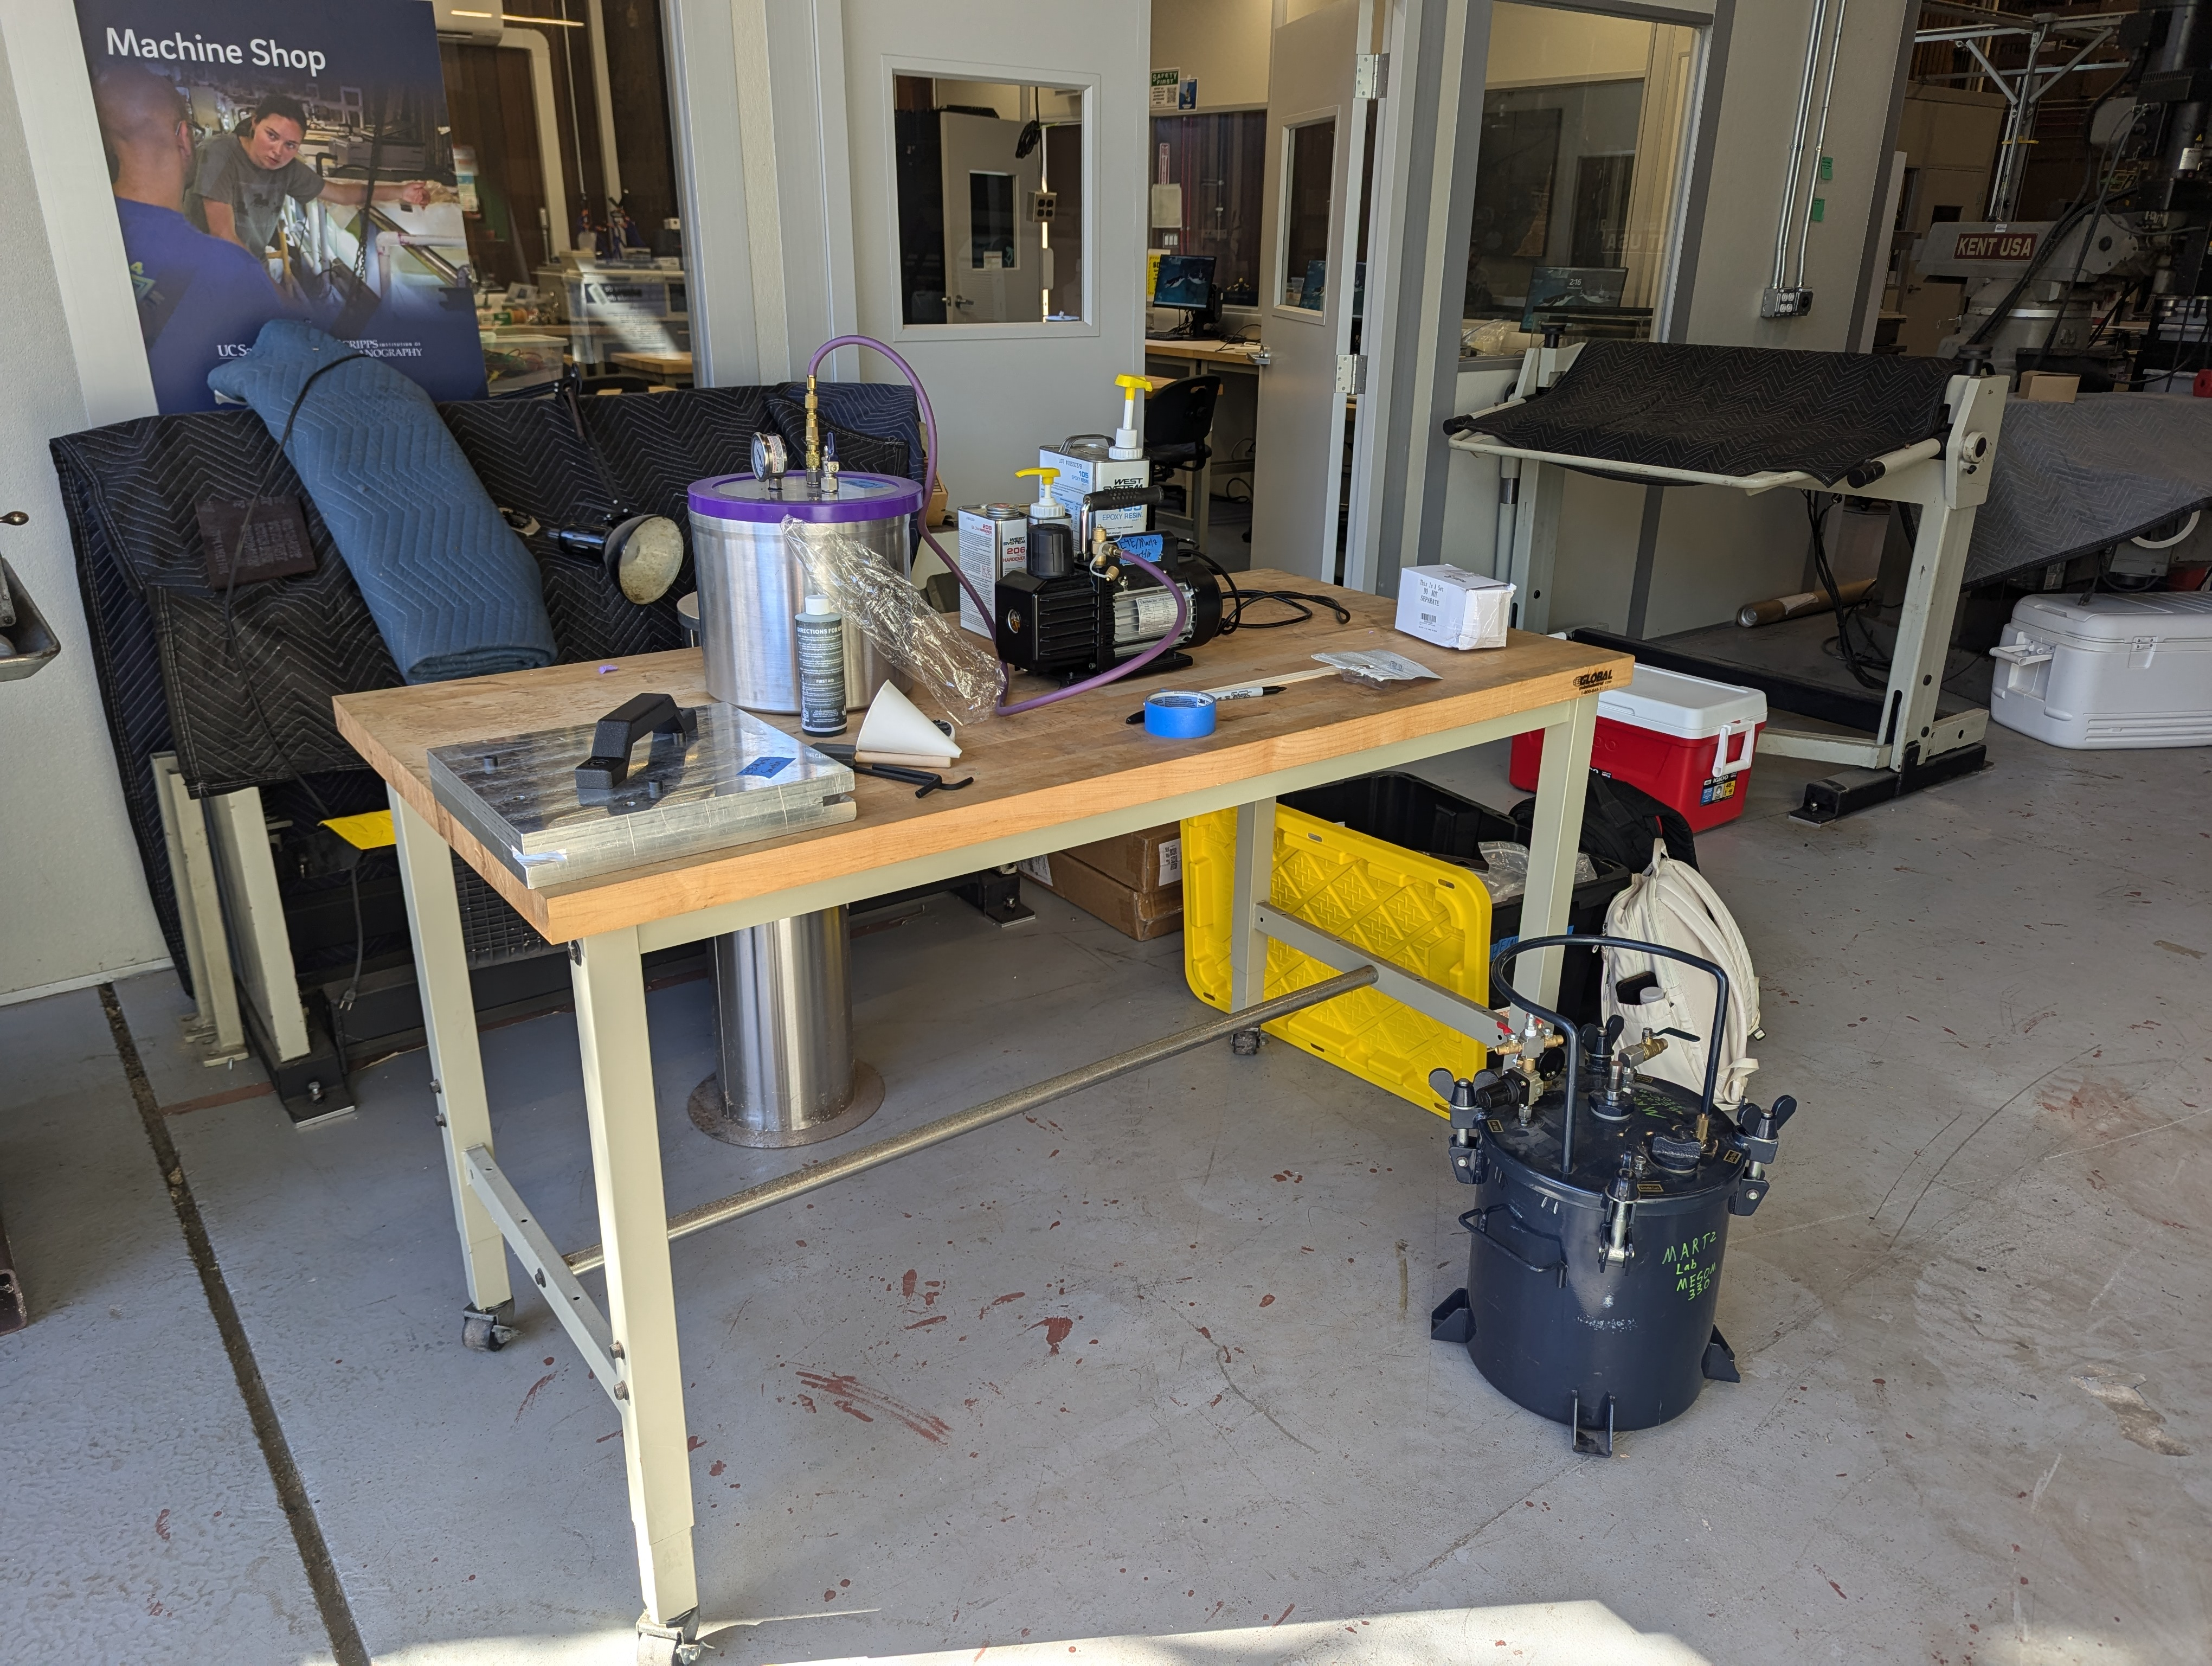
\includegraphics[width=0.9\textwidth,height=0.9\textheight,keepaspectratio]{images/sf_potting_setup.jpg}
        \end{column}
    \end{columns}
\end{frame}
% To create a slide with a bullet list, use the following:
% \begin{frame}{TITLE}
%     \begin{itemize}
%         \item ITEM 1
%         \item ITEM 2
%     \end{itemize}    
% \end{frame}

% To create a slide with numbered list, use the following:
% \begin{frame}{TITLE}
%     \begin{enumerate}
%         \item ITEM 1
%         \item ITEM 2
%     \end{enumerate}
% \end{frame}

% To create a slide with a graphic:
% 1. Add the graphic to this folder (named picture.png)
% 2. Use the following:
% \begin{frame}{TITLE}
%     \centering
%     \includegraphics[height=0.7\textheight,width=0.7\textwidth,keepaspectratio]{picture.png}
% \end{frame}

% To create a slide with two columns, use the following:
% \begin{frame}{TITLE}
%     \begin{columns}
%         \begin{column}{0.5\textwidth}
%             COLUMN 1 BODY
%         \end{column}
%         \begin{column}{0.5\textwidth}
%             COLUMN 2 BODY
%         \end{column}
%     \end{columns}
% \end{frame}
